\documentclass{book}


\usepackage{graphicx}
\usepackage[hidelinks]{hyperref}
\usepackage{fontspec}
\usepackage{amsmath}
\usepackage{amsfonts}
\usepackage{amssymb}
\usepackage{pdfpages}
\usepackage{xepersian}



\makeatletter
\renewcommand\thesection{\@arabic\c@section.\@arabic\c@chapter}
\makeatother
\makeatletter
\renewcommand\thesubsection{\@arabic\c@subsection.\@arabic\c@section.\@arabic\c@chapter}
\makeatother

\newcommand{\subtitle}[1]{%
  \posttitle{%
    \par\large\textbf{#1}\vskip0.5em}%
}

\settextfont{x-nima.ttf}

\title{
    { 
\includegraphics[width=0.33\linewidth]{Logo BOW.png} \\
        \normalsize{دانشگاه صنعتی شریف}} \\ \vspace{1cm}
    پروژه‌ی صرافی ارز دیجیتال: پایگاه داده - فاز اول \\ \vspace{0.5cm} \large{استاد: دکتر مهدی آخی} \\
    \vspace{1cm} {شمارۀ تیم: 14}}
\date{\vspace{1cm} بهار 1403}
\author{
  مانی ابراهیمی\\
  {401170491}
  \and
  محمدامین حیدری\\
  {401170553}
  \and
  محمد جعفری‌پور\\
  {401105797}
}


\def\ojoin{\setbox0=\hbox{$\bowtie$}%
  \rule[-.02ex]{.25em}{.4pt}\llap{\rule[\ht0]{.25em}{.4pt}}}
\def\leftouterjoin{\mathbin{\ojoin\mkern-5.8mu\bowtie}}
\def\rightouterjoin{\mathbin{\bowtie\mkern-5.8mu\ojoin}}
\def\fullouterjoin{\mathbin{\ojoin\mkern-5.8mu\bowtie\mkern-5.8mu\ojoin}}

\begin{document}
\maketitle
\newpage

\tableofcontents
\newpage

\chapter{کلیت فاز اول پروژه}

\section{شرح}
در این فاز تلاش شده تا یک پایگاه داده‌ی مرتبط با یک صرافی ارز دیجیتال طراحی شود. این پایگاه داده شامل موجودیت‌هایی مانند کاربر و کیف پول و تراکنش است. همچنین برای هر موجودیت روابطی با موجودیت‌های دیگر نیز تعریف شده است. در ادامه به توضیح هر یک از موجودیت‌ها و روابط آن‌ها با موجودیت‌های دیگر پرداخته‌ایم. همچنین در انتها پاسخ به 10 پرسش جبر رابطه‌ای داده شده نیز آمده است. مخزن یا همان \lr{repository} این پروژه در \href{https://github.com/maniebra/dbms-exchange-project}{\underline{اینجا}}\footnote{در صورتی که لینک برای شما کار نمی‌کند، از آدرس \lr{https://github.com/maniebra/dbms-exchange-project} استفاده نمایید.} قابل مشاهده است.

\section{تقسیم وظایف}
تیم این پروژه متشکل از سه نفر بود که برای سادگی در سند تقسیم وظایف، برای آن‌ها از اسم کوتاه استفاده کردیم:

\begin{table}[h]

    \centering
    \begin{tabular}{|c|c|c|}
        \hline
        نام کوتاه      & نام کامل       & شماره دانشجویی \\\hline
        \lr{Mani}      & مانی ابراهیمی  & 401170491      \\\hline
        \lr{Mamadamin} & محمدامین حیدری & 401170553      \\\hline
        \lr{Mamal}     & محمد جعفری‌پور  & 401105797      \\\hline
    \end{tabular}
    \caption{جدول اعضای تیم در جدول تقسیم وظایف}
\end{table}

جدول تقسیم وظایف نیز از \href{https://docs.google.com/spreadsheets/d/1x1Guh4HTWLyG9GTomZEtesp5cjIGez9m9Day3bS_kgM/edit?usp=sharing}{\underline{اینجا}}\footnote{در صورتی که این لینک برای شما کار نمی‌کند، میتوانید از آدرس \\\scriptsize\lr{https://docs.google.com/spreadsheets/d/1x1Guh4HTWLyG9GTomZEtesp5cjIGez9m9Day3bS\_kgM/edit?usp=sharing}\small\\ استفاده نمایید.} قابل مشاهده است.
\chapter{دیاگرام های \lr{ER}}
\section{شرح}
در این بخش تلاش بر این بود که کلیت پایگاه داده‌ی مورد نظر را با استفاده از دیاگرام‌های \lr{ER} نمایش دهیم. ابتدا دیاگرام \lr{ER} اصلی را نمایش داده‌ایم و سپس به تفکیک بخش‌های مختلف آن پرداخته‌ایم.
\section{توضیح هر موجودیت}
در ادامه، برای هر موجودیت حاضر در این دیاگرام توضیحی آمده:

\subsection{\lr{User}}
موجودیت کاربر یا همان \lr{user}، که دارای صفات گفته شده از جمله نام و نام خانوادگی و شناسه ملی و شماره تماس و ایمیل و رمز عبور و سایر موارد است. این موجودیت برای کاربران اصلی‌ترین موجودیت بوده چرا که اطلاعات خود هر کاربر را در این موجودیت ذخیره می‌کنیم. همچنین به یک موجودیت کیف پول متصل است که باعث می‌شود هر کاربر یک کیف پول داشته باشد.

\subsection{\lr{Wallet}}
موجودیت کیف پول یا همان \lr{wallet}، که دارای صفات گفته شده از جمله موجودیت کاربر و موجودی و ارز و سایر موارد است. این موجودیت برای ذخیره‌ی اطلاعات مربوط به کیف پول هر ارز از هر کاربر استفاده می‌شود. همچنین به یک موجودیت تراکنش متصل است که باعث می‌شود هر کیف پول دارای تراکنش باشد.

\subsection{\lr{Transactions}}
موجودیت تراکنش یا همان \lr{transactions}، که دارای صفات گفته شده از جمله موجودیت کیف پول و نوع تراکنش و مبلغ و تاریخ و سایر موارد است. این موجودیت برای ذخیره‌ی اطلاعات مربوط به تراکنش‌های هر کیف پول استفاده می‌شود. در هر تراکنش مقداری ارز از کیف پول یک کاربر خارج شده و به کیف پول کاربری دیگر می‌رود. در نظر داشته باشید که هر تبادل، دو تراکنش است.

همچنین صفت \lr{fee} در تراکنش با داشتن \lr{Market\_id} و بدست آوردن ارز پایه‌ی آن مارکت و قیمت لحظه‌ای آن ارز پایه به ریال محاسبه می‌شود.



\subsection{\lr{Orders}}
موجودیت سفارش ها یا همان \lr{Orders}، که دارای صفات گفته شده از جمله تاریخ و وضعیت و نوع ارز و حجم و قیمت و سایر موارد است. این موجودیت برای ذخیره اطلاعات مربوط به سفارشات کاربران می باشد و دارای دو نوع خرید و فروش می باشد. همچنین به یک موجودیت تبادل متصل است در اصل ترکیب دو سفارش خرید و فروش می باشد.




\subsection{\lr{Trades}}
موجودیت تبادل ها یا همان \lr{Trades}، که دارای صفات گفته شده از جمله تاریخ و حجم و مقدار و سایر موارد است. این موجودیت برای ذخیره اطلاعات مربوط به تبادل ها می باشد که تبادل ها میتواند بین یک کاربر و ادمین سایت و یا دو کاربر باشد که به ترتیب دو موجودیت \lr{OTC} و  \lr{P2P}رو تشکیل داده اند. همچنین این موجودیت دارای یک شناسه برای هر تبادل می باشد. صفت \lr{\texttt{min\_fill\_remainder}} به این صورت عمل می‌کند که حجم باقی‌مانده‌ی کمینه‌ی دو سفارش خرید و فروش را ذخیره می‌کند.

\subsubsection{\lr{OTC}}
شامل \lr{ID} ادمین و مشتری می‌باشد که بوسیله‌ی شناسه‌ی \lr{Market} به بازار مربوطه متصل شده است.

\subsubsection{\lr{P2P}}
شامل دو \lr{ID} و \lr{OrderID} خریدار و فروشنده یا همان \lr{maker} و \lr{taker} می‌باشند که به وسیله‌ی شناسه‌ی صرافی یا همان \lr{Broker\_ID} به صرافی مربوطه متصل شده‌اند.



\subsection{\lr{OrderBooks}}
موجودیت لیست سفارشات یا همان \lr{OrderBooks}، که دارای صفات گفته شده از جمله شناسه و  شناسه ی بازار و و سایر موارد است. این موجودیت برای ذخیره اطلاعات مربوط به لیست های سفارشات هر فروشگاه میباشد، همچنین به یک موجودیت لیست که زیرمجموعه‌ی \lr{OrderBooks} است متصل شده که شامل دو نوع لیست خرید و فروش می باشد و به موجودیت سفارشات که خود دو نوع خرید و فروش دارد نیز متصل است که در نهایت این دو نوع خرید و فروش با هم سفارشات را بتواند بسازد.






\subsection{\lr{Markets}}
موجودیت فروشگاه ها یا همان \lr{Markets}، که دارای صفات گفته شده از جمله کارمزد و  قیمت لحظه ای بازار و نوع ارز پایه و سایر موارد است. این موجودیت برای ذخیره اطلاعات مربوط به فروشگاه های خرید و فروش ارز دیجیتال برای کاربران می باشد. همچنین به یک موجودیت لیست سفارشات متصل است که شامل دو لیست خرید و فروش هر فروشگاه می باشد.







\subsection{\lr{Brokers}}
موجودیت صرافی ها یا همان \lr{Brokers}، که دارای صفات گفته شده از جمله شناسه و سایر موارد است. این موجودیت برای ذخیره اطلاعت مربوط به صرافی های ارز دیجیتال می باشد. همچنین به موجودیت فروشگاه ها متصل می باشد که برای هر ارز پایه در صرافی یک فروشگاه وجود دارد و به یک یا چند \lr{admin} متصل است که در ان ادمین های هر صرافی مشخص می شوند.
\subsection{\lr{CryptoCurrency}}
موجودیت کریپتو ها یا\lr{CryptoCurrency}   ارز هایی اند که در سایت وجود دارند و توسط افراد مبادله میشوند. این ارز ها ممکن است قیمت ثابت \lr{Stable coin}باشند و یا قیمت انها هرلحظه عوض شود \lr{nonstable Currency}.

\subsection{\lr{Network}}

هر ارز شامل چندین شبکه ی مجزا از هم است که تراکنشهای آنها روی بستر متفاوتی انجام میشود.این شبکه ها دارای کارمزد و زمان متفاوتی اند.

\subsection{\lr{Online Payments}}
تاریخچه‌ی تمامی واریزی‌های هر کاربر، مقدار آن و زمان انجام‌شده است.


\subsection{\lr{Wallet History}}
تاریخچه‌ای از تغییرات میزان هر کیف پول است و هر تراکنشی برای دو کیف پول یک \lr{Wallet History} جدید می‌سازد.


\subsection{\lr{Crypto Histories}}
تاریخچه‌ی تغییرات قیمت یک رمزارز است که زمان آن تغییر و مقدار و قیمت آن در آن زمان (قیمت همان قیمت لحظه‌ای مارکت است) نشان می‌دهد. با انجام هر تراکنش یک \lr{CryptoHistory} جدید ایجاد می‌شود چرا که قیمت لحظه‌ای ارز تغییر می‌کند.




\chapter{سوالات جبر رابطه‌ای}
\section{شرح}
در این بخش پاسخ به 10 سوال جبر رابطه‌ای\footnote{\lr{Relational Algebra}} آمده است.
\section{پاسخ به سوالات}
\subsection{سوال 1}

$\Pi_{market\_id, fee}(Transactions \\ \bowtie_{Transactions.market\_id = Market.market\_id \land Transactions.date = date}(\\
    _{market\_id}\mathcal{F}_{\max (date)} (\\
    Market \bowtie_{Market.market\_id = Transactions.market\_id} Transactions)))$

\subsection{سوال 2}
$$_{owner\_id}\mathcal{F}_{\mathtt{Sum}(total\_value \times in\_time\_price)} [ Wallets \bowtie_{Market.market\_id = id} Markets]$$

\subsection{سوال 3}
$$_{crypto\_id} \mathcal{F}_{\mathtt{Count}(order\_id)} [\sigma_{fill = "false"} (Orders)]$$

\subsection{سوال 4}

$A = \rho_{user\_id, total}[ _{owner\_id} \mathcal{F}_{\mathtt{Sum}(fee) as totalSell} \newline(
    Transactions \bowtie_{Transactions.origin\_wallet\_id = wallets.id} Wallet
    )]$\\
$B = \rho_{user\_id, total}[ _{owner\_id} \mathcal{F}_{\mathtt{Sum}(fee) as totalBuy} \newline(
    Transactions \bowtie_{Transactions.dest\_wallet\_id = wallets.id} Wallet
    )]$
$$_{user\_id}\mathcal{F}_{\mathtt{Sum}(Total)}$$


\subsection{سوال 5}

$A = _{user\_id, cryptoid} \mathcal{F}_{\mathtt{Count}(Transactions.id)}(\\(Users \times Cryptocurrency) \ltimes_{users.user\_id = Transactions.SellerID} \\Transactions)$\\

$B = _{user\_id, cryptoid} \mathcal{F}_{\mathtt{Count}(Transactions.id)}(\\(Users \times Cryptocurrency) \ltimes_{users.user\_id = Transactions.BuyerID}\\ Transactions)$\\
\quad\\
$_{user\_id, cryptoid} \mathcal{F}_{mathtt{Sum}(TotalCount)} (\\\rho_{user\_id, cryptoid/ TotalCount(A)} \cup \rho_{user\_id, cryptoid/ TotalCount(B)} )$

\subsection{سوال 6}
$$\mathcal{F}_{\mathtt{Sum}(fee)}[\sigma_{Now-Date \geq "0000-00-30-00:00:00"}(Transactions)]$$

\subsection{سوال 7}

\begin{latin}

    $A= \Pi_{cryptoid, in\_time\_price} (Cryptocurrency)$\\
    $B=_{cryptoid} \mathcal{F}_{mathtt{max}(Date) as Date} (\\\sigma_{Transactions.Date - Now() \leq "0000-00-30-00:00:00"}(Transactions \rtimes Cryptocurrency))$\\
    $C = \Pi_{cryptoid,fee} [Cryptocurrency \bowtie_{Cryptocurrency.id Transactions.cryptoid} (\\Transactions \bowtie B)]$
    $$\Pi_{cryptoid, in\_time\_price - fee} (A \bowtie) C$$
\end{latin}


\subsection{سوال 8}

\begin{latin}
    $A = _{owner\_id} \mathcal{F}_{\mathtt{Sum}(Total\_value) as sum} (Wallets)$\\
    $B = \Pi_{owner\_id, cryptoid, Total\_value} (Wallets)$\\
    $_{cryptoid}\mathcal{F}_{\mathtt{count}(owner\_id)} [\sigma_{percentage \geq 0.05} (\rho_{cryptoid, owner\_id, percentage}[\\\Pi_{cryptoid, owner\_id, \frac{Total\_value}{Sum}(A\bowtie B)}])]$
\end{latin}


\subsection{سوال 9}

\begin{latin}
    $A = \Pi_{user\_id, Date} (\sigma_{Date - Now() \leq "0000-00-30;00:00:00"}(Online\_Payments))$\\
    $B = \rho_{user\_id, paymentDate}(A) \bowtie WalletHistories$\\
    $C =_{cryptoid, user\_id, paymentDate}\mathcal{F}_{\mathtt{Max}(Date)} (\sigma_{Date < paymentDate}(B))$\\
    $\rho_{user_id, paymentDate}(A) \times CryptoHistories$\\
    $E = _{cryptoid, user\_id, paymentDate}\mathcal{F}_{\mathtt{max}(Date)}(\sigma_{Date < paymentDate} (D))$\\
    $X = _{user\_id, paymentDate}\mathcal{F}_{\mathtt{Sum}(amount \times price) as totalValue} ((C \times WalletHistories) \\\bowtie_{user\_id = user\_id \land paymentDate = paymentDate} E \bowtie CryptoHistories) \\\bowtie_{user\_id = user\_id \land paymentDate = paymentDate} Online\_Payments$\\
    $$\mathcal{F}_{\mathtt{CountUnique(user\_id)}}(\sigma_{onlineamount \geq \frac{1}{5} totalValue} (X))$$
\end{latin}


\subsection{سوال 10}
$A = \rho_{cryptoid, price, totalSell} [_{cryptoid, price}\mathcal{F}_{\mathtt{Sum(amount)}}((Cryptocurrency \times prices) \\\bowtie_{Cryptocurrency.id = sellOrders.cryptoid} sellOrders)]$\\
$B = \rho_{cryptoid, price, totalSell} [_{cryptoid, price}\mathcal{F}_{\mathtt{Sum(amount)}}((Cryptocurrency \times prices) \\\bowtie_{Cryptocurrency.id = purchaseOrders.cryptoid} purchaseOrders)]$\\
$$A \cup B$$

\chapter{ضمیمه: تصویر دیاگرام \lr{ER}}
در انتهای فایل، ضمیمه‌ی تصویر دیاگرام مربوطه آمده است.

در صورتی که در مشاهده‌ی این تصویر مشکل دارید، فایل \lr{PDF} را با مرورگرهای \lr{Edge} یا \lr{Chrome} باز نمایید.


\includepdf[pages=-]{./erds/erd.pdf}
\chapter{کلیت فاز دوم پروژه}
\section{شرح}
ما در این فاز از پروژه چهار تِغیر در نموار فاز قبلی خود ایجاد کردیم که به ترتیب عبارتند از بهینه کردن نمودار برای طراحی دیتابیس، ایجاد دیتابیس، نرمال سازی و ایندکس کردن دیتا بیس و در نهایت انجام هشت جستوجو در دیتابیس.
\chapter{تبدیل نمودار‌های‌‌ فاز اول، به نمودار‌های منطبق با \lr{SQL}}
\section{چهار تغیر در نمودار برای بهینه سازی}
\newpage

\subsection{رابطه ی چند به چند بین کیف پول و تراکنش‌ها}
از انجایی که در هر تراکنش دو کیف پول استفاده میشد و هر کیف پول در چندین تراکنش شرکت میکرد، یک جدول جدید اضافه کردیم که رابطه ی چند به چند را به دو رابطه ی یک به چند تقسیم کند.

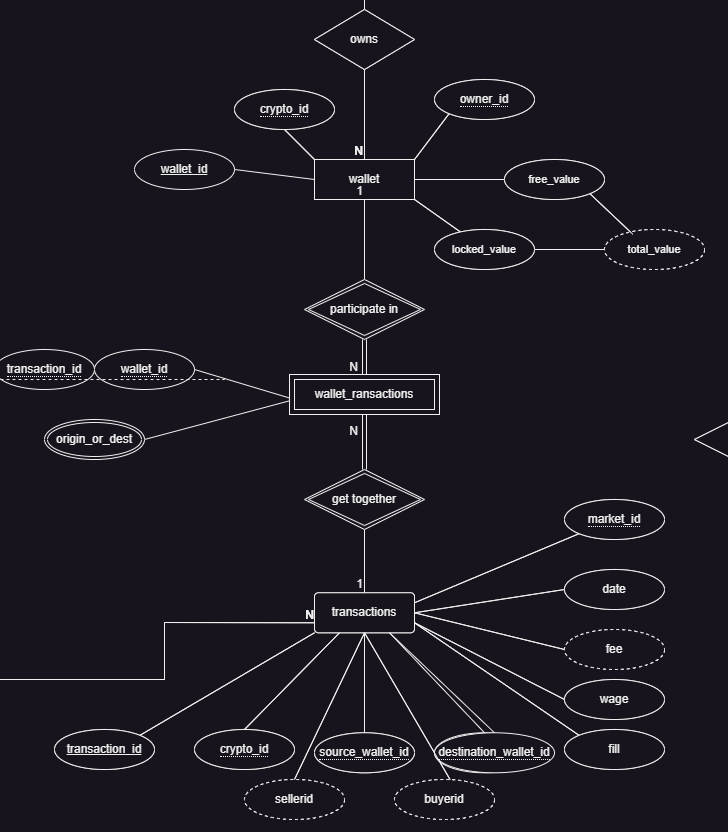
\includegraphics[width=0.8\linewidth]{wallets_transactions.png}
\newpage

\subsection{رابطه ی چند به چند بین کاربرها و تبادل ها}
از انجایی که هر تبادل از دو کاربر و هر کاربر در چندین تبادل شرکت میکرد، یک جدول جدول جدید اضافه کردیم که رابطه ی چند به چند را به دو رابطه ی یک به چند تسیم بکمد.

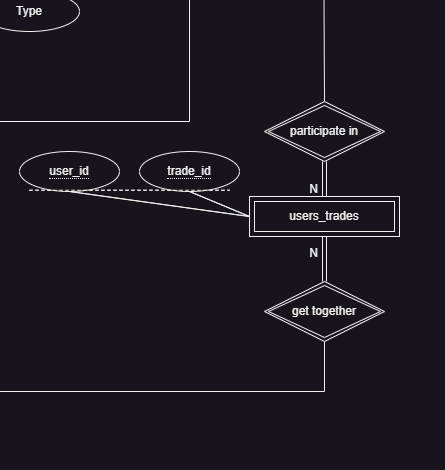
\includegraphics[width=0.8\linewidth]{users_trades.png}
\newpage

\subsection{رابطه ی اسپیسیفیکیشن در سفارشات}
در فاز قبلی سفارشات به دو دسته‌ی سفارشت خرید و سفارشات فروش تقسیم می‌شدند که ما در این فاز ای رابطه را در یک جدول سفارشات از طریق ستونی به نام \lr{type} تفکیک کرده ایم.

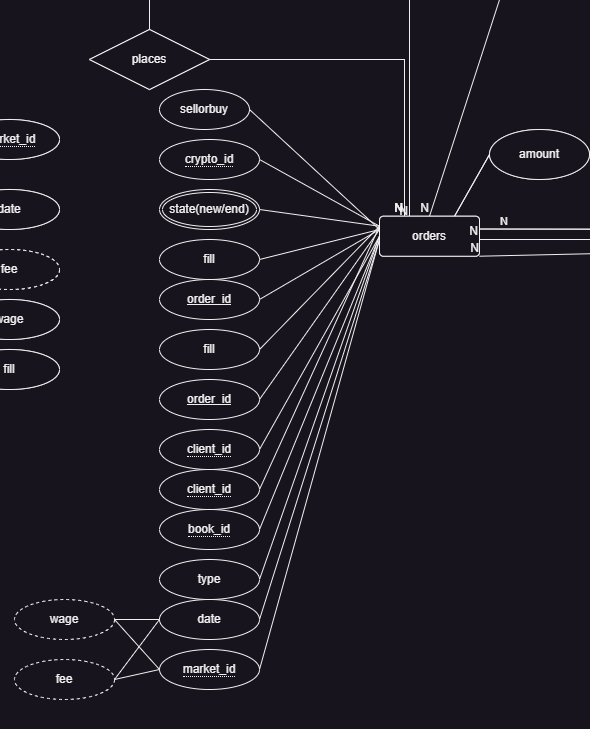
\includegraphics[width=0.8\linewidth]{orders.png}
\newpage

\subsection{رابطه ‌ی جنرالیزیشن در تبادل‌ها}
در فاز قبلی تبادل‌ها شامل دو نوع \lr{p2p} و \lr{otc} می‌شدند که ما در این فاز آن دو نوع تبادل را در یک جدول تبادل قرار دادیم که با ستون \lr{type} از هم تفکیک می شوند.

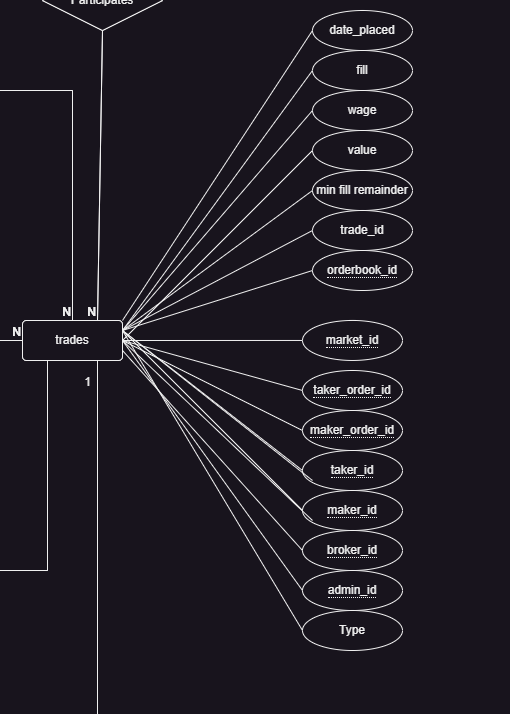
\includegraphics[width=0.8\linewidth]{trades.png}
\newpage

\end{document}
